\chapter{Systembeskrivelse}
Systemet, der er blevet udviklet er en blodtryksmåler. Blodtryksmåleren er tiltænkt at fungere som en invasiv blodtryksmåler på operationsstuer, der skal monitorerer patienters blodtryks under operationer.\\

\begin{figure}[H]
	\centering
	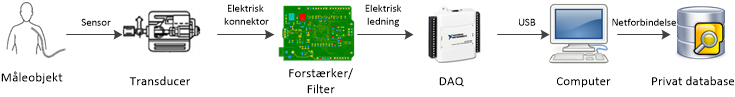
\includegraphics[width=1\textwidth]{Figurer/Systembeskrivelse}
	\caption{Forsøgsopstilling grafisk}
	\label{opstilling}
\end{figure} 
For at kunne lave et sådan system er der blevet udviklet en hardware del og en software del. 
Hardwaredelen modtager det fysiske tryk fra måleobjektet gennem en transducer, hvis funktion er at omdanne trykket til et elektrisk signal med enheden mV.\\
Hardwaren er bestående af en forstærker, og et filter, hvor signalet først forstærkes håndterbart område, der er anvendeligt i DAQ'en. Desuden består systemet også af et analogt lavpas filter, som filtrerer og frasorterer frekvenser på 50Hz og opefter.\\
Efter endt filtrering konverteres det analoge signal i DAQ'en til et digitalt signal, der er håndterbart i softwaren\\[1ex]

Softwaren er det program, som skal monitorere der digitale signal grafisk. Programmet er bestående af en brugergrænseflade, program og adgang til en privat database. Brugergrænsefladen viser et digitalt signal via programmet og giver brugeren mulighed for at benytte forskellige funktioner og indhente oplysninger. Gennem programmets funktioner har brugeren mulighed for at foretage en digital filtrering af blodtrykssignalet aflæse systolen, diastolen og aflæse pulsen.\\
 Før brugeren får adgang til blodtryksmålingen skal der foretages en nulpunktjustering, samt en tekniker har mulighed for at foretage en årlig kalibrering, gennem et login-vindue. Systemet kan desuden efter endt måling lagre data fra blodtryksmålingen i en privat database.\\[1ex]

Projektets endelige produkt er en prototype af et blodtryksmålings system, som kan benyttes til invasiv blodtryksmåling.


